\section{Modélisation UML}
\label{sec:uml}

% todo: Avant le cours relire les chapitres 3, 4, 5 et 11.

\begin{frame}
    \frametitle{Définition}
    \begin{columns}
        \begin{column}{0.5\textwidth}
            Le langage de modélisation unifié (UML) est une famille de \textbf{notations graphiques},
            soutenues par un méta-modèle unique,
            qui aident \underline{à décrire et à concevoir} des systèmes logiciels,
            en particulier des systèmes logiciels construits à l'aide du style orienté objet.
        \end{column}
        \begin{column}{0.5\textwidth}
            \centering
            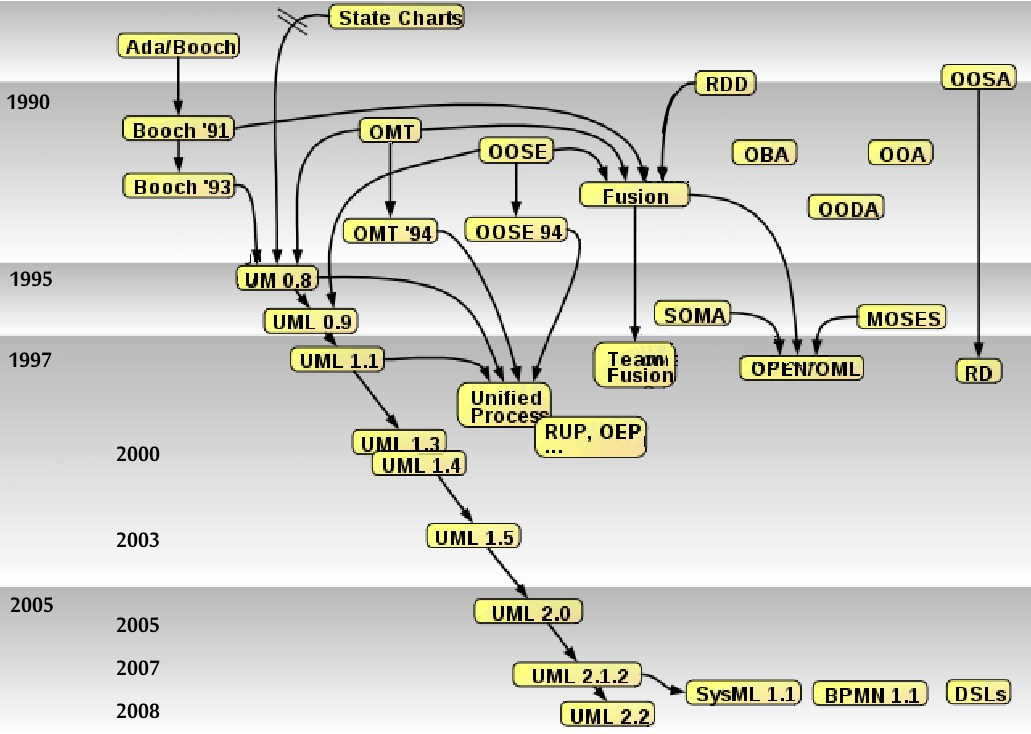
\includegraphics[width=\linewidth]{figures/uml/uml-historie}
        \end{column}
    \end{columns}
\end{frame}

\begin{frame}
    \frametitle{Les diagrammes}
    \begin{itemize}
        \item Diagrammes de structure
        \item Diagrammes de comportement
    \end{itemize}
    \centering
    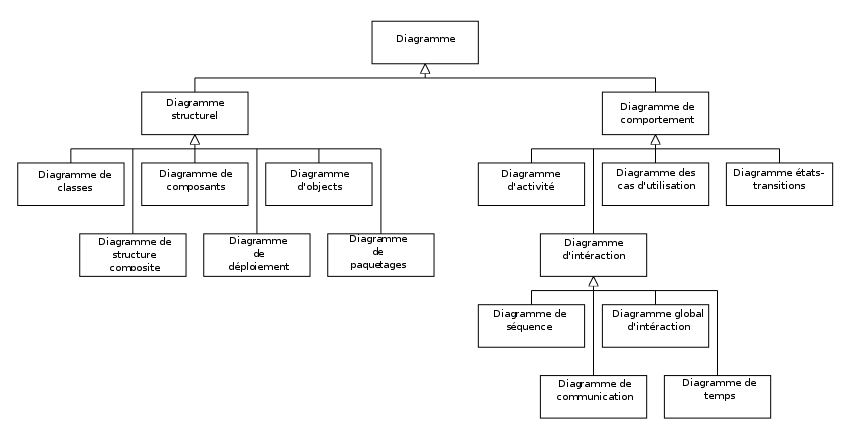
\includegraphics[height=0.4\linewidth]{figures/uml/uml-diagrammes}
\end{frame}

\subsection{Diagramme de classes}
\label{subsec:diagramme-classes}

\begin{frame}
    \frametitle{Diagramme de classes}
    Un diagramme de classes \textbf{décrit les types d'objets du système}
    et les différents types de \underline{relations statiques} qui existent entre eux.
    Les diagrammes de classes montrent également
    \emph{les propriétés et les opérations} d'une classe
    ainsi que les contraintes qui s'appliquent à la manière dont les objets sont connectés.
\end{frame}

\begin{frame}
    \frametitle{Une classe}
    \centering
    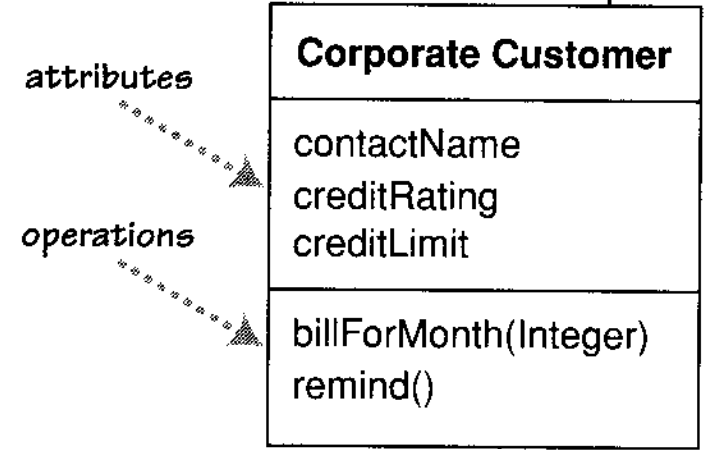
\includegraphics[height=0.5\linewidth]{figures/uml/classe}
\end{frame}

\begin{frame}
    \frametitle{La généralisation (héritage)}
    \centering
    \includegraphics[height=0.5\linewidth]{figures/uml/classe-héritage}
\end{frame}

\begin{frame}
    \frametitle{Un diagramme de classes simple}
    \centering
    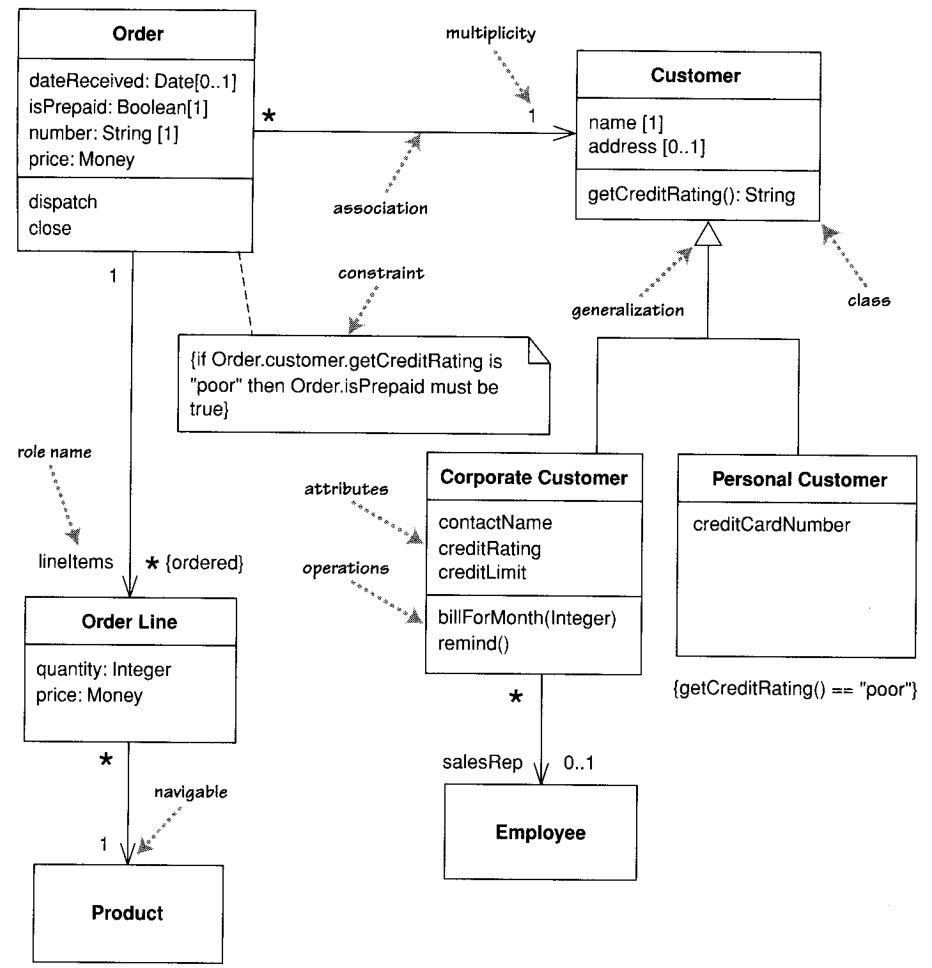
\includegraphics[height=0.5\linewidth]{figures/uml/classe-complet}
\end{frame}

\begin{frame}
    \frametitle{Les propriété comme association ou attribut ?}
    \centering
    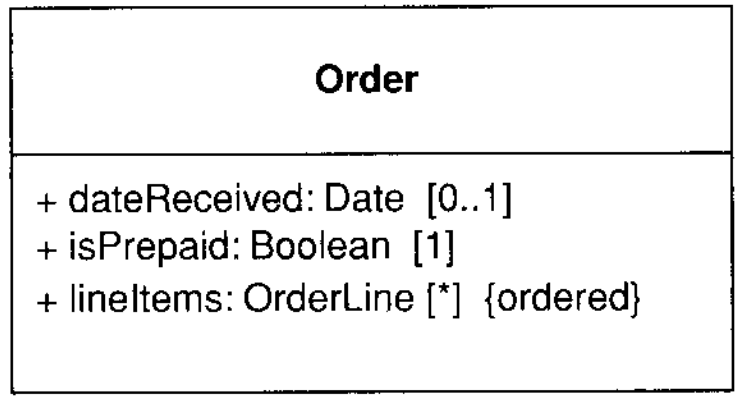
\includegraphics[height=0.15\linewidth]{figures/uml/classe-propriétés-1}
    \vfill
    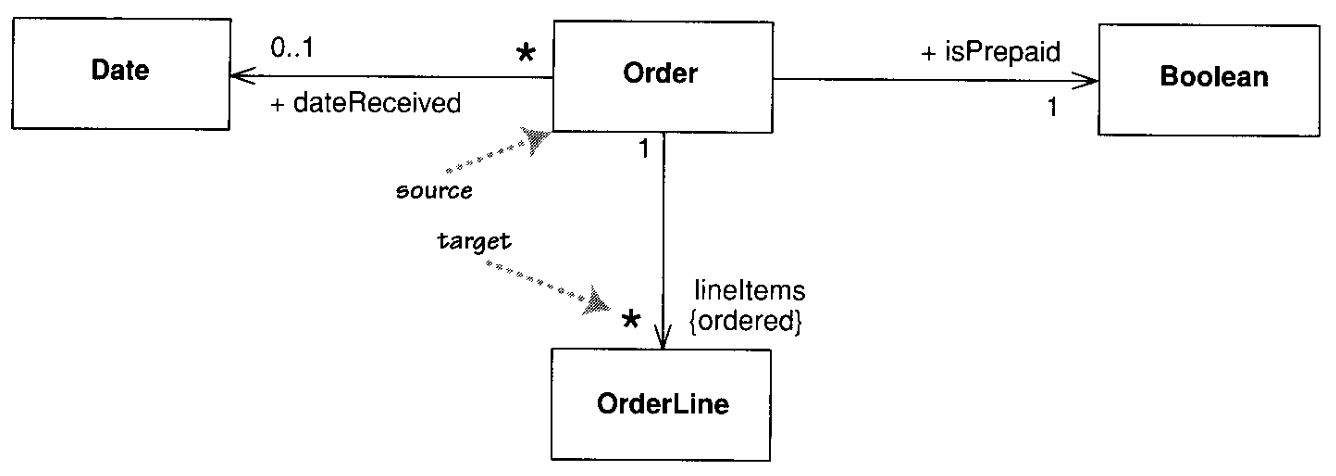
\includegraphics[height=0.25\linewidth]{figures/uml/classe-propriétés-2}
\end{frame}

\begin{frame}
    \frametitle{Cardinalité et directionnalité}
    \begin{itemize}
        \item \textbf{Optionnel} implique une limite inférieure de 0 ;
        \item \textbf{Obligatoire} implique une limite inférieure de 1 ou éventuellement plus ;
        \item \textbf{Une valeur unique} implique une limite supérieure de 1 ;
        \item \textbf{Une valeur multiple} implique une limite supérieure à 1 (généralement *).
    \end{itemize}
    \vfill
    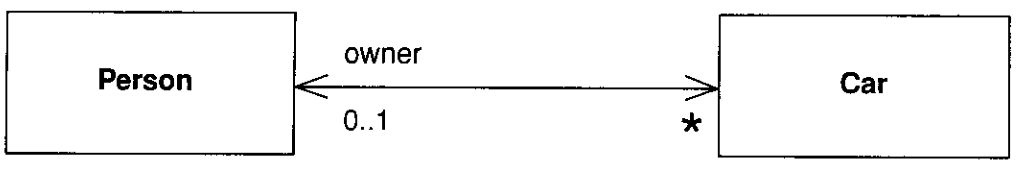
\includegraphics[width=\textwidth]{figures/uml/classe-bidirectionnelle}
\end{frame}

\begin{frame}
    \frametitle{Dépendance}
    Une dépendance existe entre deux éléments si des
    modifications de la définition d'un élément (le fournisseur)
    peuvent entraîner des modifications de l'autre (le client).
    \vfill
    \includegraphics[width=\textwidth]{figures/uml/classe-dépendance}
\end{frame}

\begin{frame}
    \frametitle{Agrégation et composition}
    \centering
    \includegraphics[width=\textwidth]{figures/uml/classe-agrégation-composition}
\end{frame}

\begin{frame}
    \frametitle{Implémentation}
    \centering
    \includegraphics[height=0.5\linewidth]{figures/uml/classe-implémentation}
\end{frame}

\begin{frame}
    \frametitle{Diagrammme de classes PlantUML}
    \begin{columns}
        \begin{column}{0.4\textwidth}
            \lstinputlisting[
                basicstyle=\tiny,
                label=lst:classe-plantuml]
            {figures/uml/classe-plantuml.puml}
        \end{column}
        \begin{column}{0.6\textwidth}
            \centering
            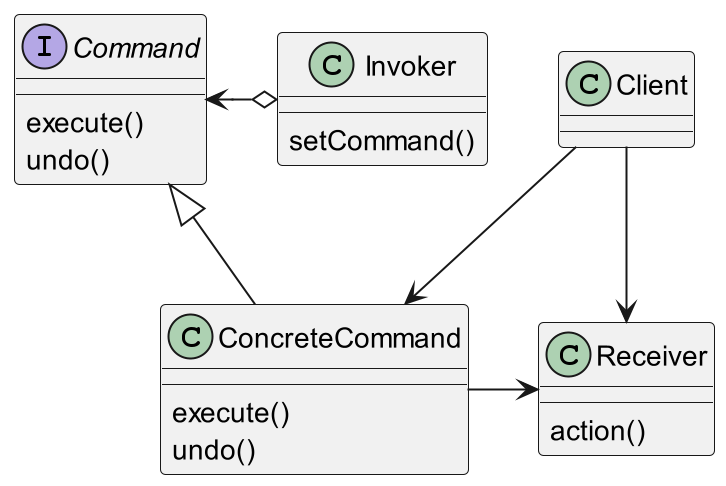
\includegraphics[width=0.8\linewidth]{figures/uml/classe-plantuml}
        \end{column}
    \end{columns}
\end{frame}

\subsection{Diagramme de séquence}
\label{subsec:diagramme-sequence}

\begin{frame}
    \frametitle{Diagramme de séquence}
    Un diagramme de séquence montre la \textbf{collaboration dynamique} entre plusieurs objets
    en décrivant \emph{l’ordre temporel} dans lequel les messages sont envoyés entre eux.
\end{frame}

\begin{frame}
    \frametitle{Un permier diagramme de séquence}
    \centering
    \includegraphics[height=0.5\linewidth]{figures/uml/sequence-exemple-centralisé}
\end{frame}

\begin{frame}
    \frametitle{Le même, mais distribué au lieu de centralisé}
    \centering
    \includegraphics[height=0.5\linewidth]{figures/uml/sequence-exemple-distribué}
\end{frame}

\begin{frame}
    \frametitle{Création et suppression des participants}
    \centering
    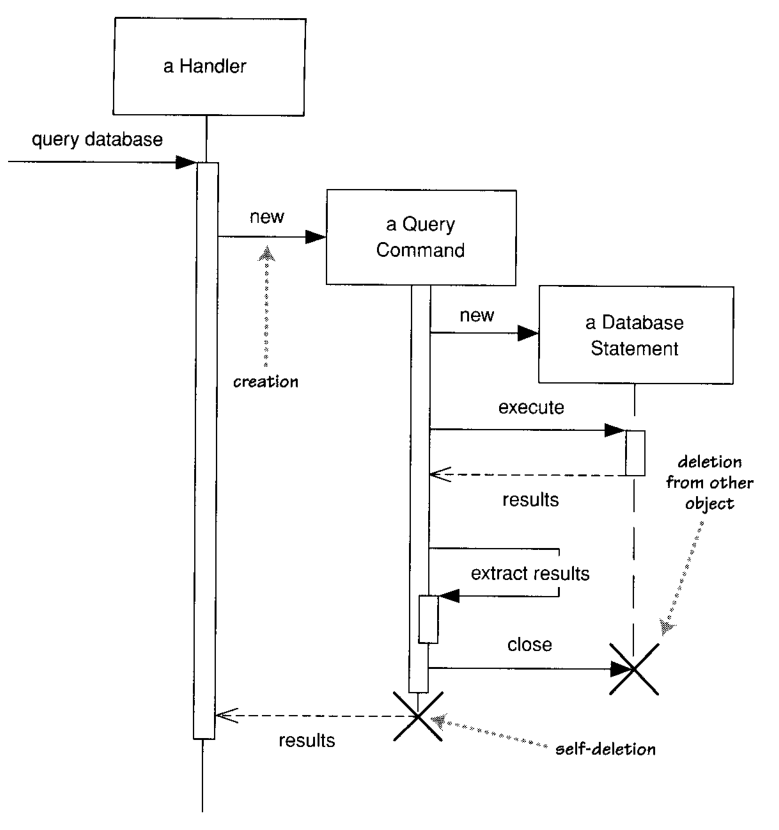
\includegraphics[height=0.5\linewidth]{figures/uml/sequence-creation-deletion}
\end{frame}

\begin{frame}
    \frametitle{Fragments : Boucles, conditions, etc}
    \centering
    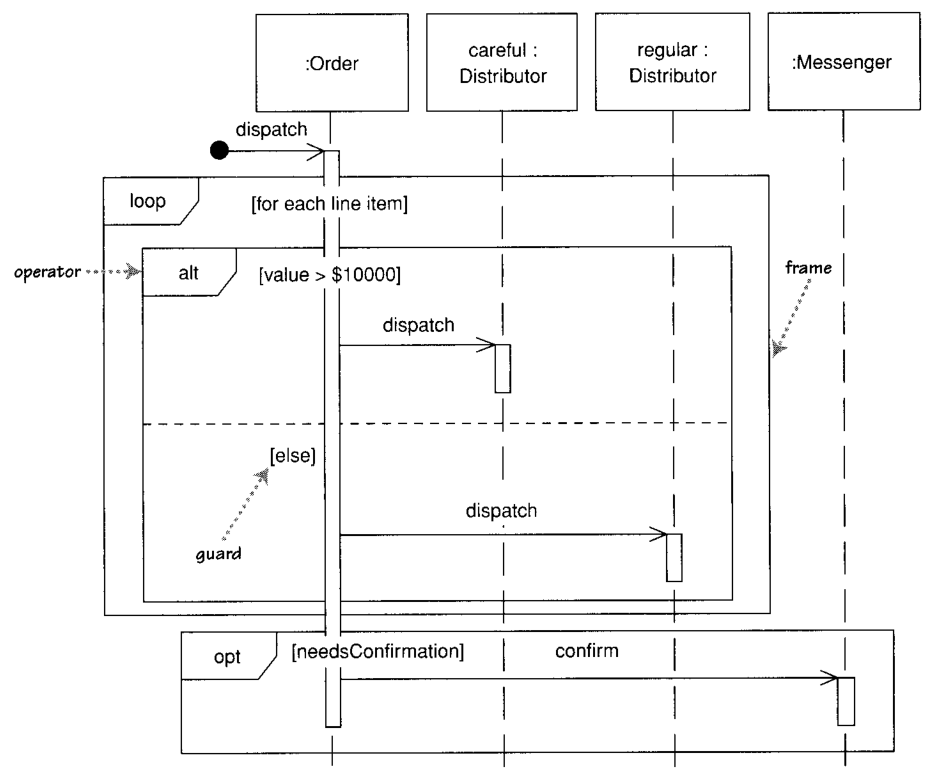
\includegraphics[height=0.5\linewidth]{figures/uml/sequence-fragments}
\end{frame}

\begin{frame}
    \frametitle{Quelques opérateurs de fragments}
    \begin{itemize}
        \item \textbf{alt} : Fragments multiples alternatifs, seulement celui dont la garde est vraie s'exécutera.
        \item \textbf{opt} : Facultatif, le fragment ne s'exécute que si la condition fournie est vrai.
        \item \textbf{par} : Parallèle, chaque fragment est traité en parallèle.
        \item \textbf{loop} : Boucle, le fragment peut s'exécuter plusieurs fois et la garde indique la base de l'itération.
        \item \textbf{ref} : Référence, fait référence à une interaction définie sur un autre diagramme.
    \end{itemize}
\end{frame}

\begin{frame}
    \frametitle{Diagramme de séquence PlantUML}
    \begin{columns}
        \begin{column}{0.4\textwidth}
            %todo: problème d'affichage du listing...
            \lstinputlisting[
                basicstyle=\tiny,
                label=lst:sequence-plantuml]
            {figures/uml/sequence-plantuml.puml}
        \end{column}
        \begin{column}{0.6\textwidth}
            \centering
            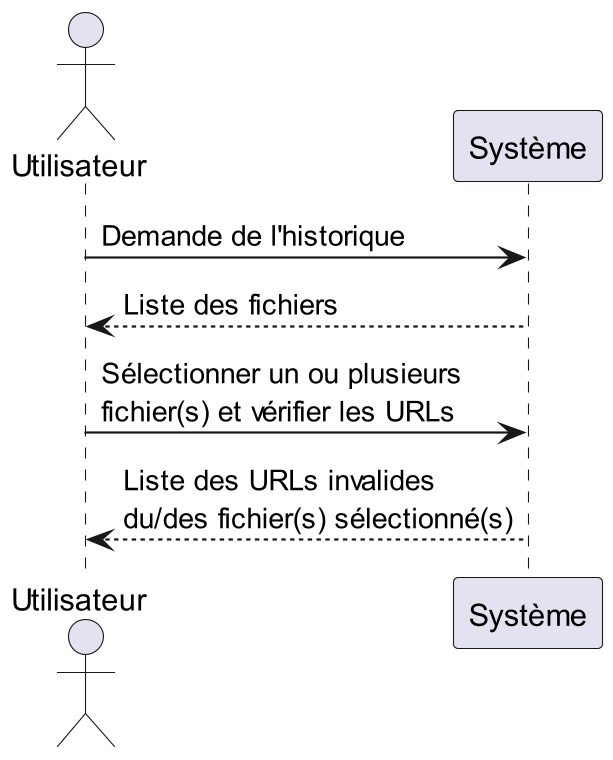
\includegraphics[height=0.8\linewidth]{figures/uml/sequence-plantuml}
        \end{column}
    \end{columns}
\end{frame}

\subsection{Diagramme d'activité}
\label{subsec:diagramme-activite}

\begin{frame}
    \frametitle{Diagramme d'activité}
    Les diagrammes d'activités sont une technique pour décrire
    la \textbf{logique procédurale}, les \textbf{processus métier} et les \textbf{flux de travail}.
\end{frame}

\begin{frame}
    \frametitle{Un exemple simple de diagramme d'activité}
    \centering
    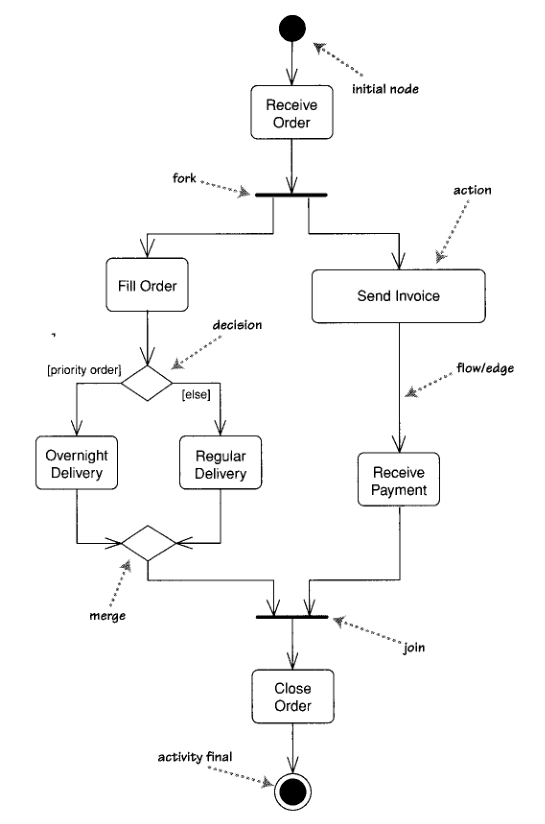
\includegraphics[height=0.5\linewidth]{figures/uml/activite-exemple}
\end{frame}

\begin{frame}
    \frametitle{Diagramme d'activité PlantUML}
    \begin{columns}
        \begin{column}{0.4\textwidth}
            %todo: problème d'affichage du listing...
            \lstinputlisting[
                basicstyle=\tiny,
                label=lst:activite-plantuml]
            {figures/uml/activite-plantuml.puml}
        \end{column}
        \begin{column}{0.6\textwidth}
            \centering
            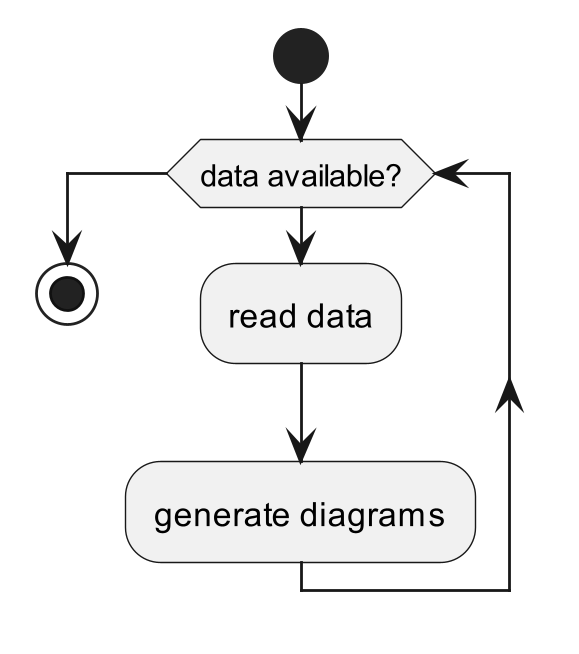
\includegraphics[height=0.8\linewidth]{figures/uml/activite-plantuml}
        \end{column}
    \end{columns}
\end{frame}

\begin{frame}
    \frametitle{Un livres de référence}
    \centering
    
\includegraphics[height=0.5\linewidth]{figures/uml/uml-book}
\end{frame}
